\chapter{Introdução}

O Brasil, como membro da Organização das Nações Unidas (ONU), comprometeu-se numa agenda a concluir dezessete Objetivos de Desenvolvimento Sustentável~\cite{odsbrasil} até 2030. Jogos são uma forma de entretenimento popular e amplamente acessível, que pode envolver jogadores em tarefas desafiadoras e educacionais. Quando usados de maneira estratégica, podem ser ferramentas poderosas para engajar a população em causas importantes, como a promoção dos Objetivos de Desenvolvimento Sustentável (ODS) estabelecidos pela ONU. Os jogos podem transmitir informações de forma interativa e envolvente, permitindo que os jogadores sejam incentivados a aprender sobre qualquer questão. Neste sentido, jogos podem servir como ferramentas de interação para atingir uma parcela da população e colaborar para o alcance desses objetivos. Além disso, campanhas conscientizadoras por meio de jogos podem incentivar comportamentos mais sustentáveis~\cite{joseamericonetoGameOds}.

\par
Visto que os problemas ambientais podem afetar diretamente os objetivos de desenvolvimento social, é importante considerar que a atualidade conta com um acelerado avanço tecnológico combinado com o descarte muitas vezes incorreto dos materiais eletrônicos produzidos, bem como dos resíduos gerados. Como consequência, essas questões nem sempre recebem a atenção que merecem. Existem várias razões pelas quais essas questões ambientais muitas vezes não recebem a atenção necessária. Algumas dessas razões incluem falta de conscientização sobre a importância do meio ambiente, falta de regulamentações e políticas públicas efetivas, interesses econômicos em conflito com a proteção ambiental, falta de recursos financeiros para investimentos em sustentabilidade, entre outras. Além disso, muitas vezes ações ambientalmente corretas requerem mudanças de comportamento e hábitos, o que pode ser difícil de implementar em larga escala.
Considerando que os recursos empregados na produção de produtos eletrônicos são limitados e que seu descarte inadequado pode provocar a contaminação de solos e lençóis freáticos \cite{eWasteContamination}, a problemática em questão se alinha com os Objetivos de Desenvolvimento Sustentável (ODS) da Organização das Nações Unidas (ONU), que buscam abordar os desafios ambientais globais e alcançar um futuro mais sustentável até 2030. Nesse sentido, a gestão adequada de resíduos eletrônicos é fundamental para garantir a preservação do meio ambiente e a promoção de um desenvolvimento sustentável em escala global.
\par
Podemos utilizar jogos sérios educativos como uma ferramenta de aprendizado para conscientização e informação sobre assuntos como o descarte de materiais eletrônicos. Além disso, esses jogos permitem apresentar sistemas complexos de um modo dinâmico, ampliando a compreensão acerca de conteúdos. Eles não se restringem a leituras ou a assistir, mas também permitem interagir, proporcionando um papel ativo ao jogador, o que os torna uma excelente forma de aprendizado. \cite{Vasconcellos_Carvalho_Barreto_Atella_2017}
\par

Pela ótica da Interação Humano-Computador, o processo de design pode auxiliar na análise da situação, síntese da intervenção e avaliação da nova situação. Temos que:
\begin{itemize}
    \item A análise da situação evidencia o compromisso assumido pelo Brasil em relação aos dezessete Objetivos de Desenvolvimento Sustentável estabelecidos pela ONU, os quais devem ser alcançados até o ano de 2030. Entretanto, há um problema ecológico preocupante relacionado à poluição gerada pelos materiais eletrônicos que tem sido negligenciado e merece atenção imediata. É importante salientar que tal problemática não foi mencionada na agenda da COP26, conforme afirmado por \cite{skelton_2021} . Dessa forma, faz-se necessário que sejam adotadas medidas efetivas para o controle e redução desse tipo de poluição, a fim de garantir o cumprimento dos objetivos estabelecidos pela ONU e a preservação do meio ambiente para as gerações futuras.
    \item A presente intervenção tem como objetivo desenvolver uma ferramenta lúdica que aborde questões climáticas e de reciclagem de materiais eletrônicos, conhecido como WEEE (\textit{Waste Electrical and Electronic Equipment}). Tal ferramenta é um jogo educativo, intitulado What Weee Are, que busca disseminar o conhecimento acerca das consequências do descarte inadequado de materiais eletrônicos e sensibilizar o público infantil sobre a importância da reciclagem e do consumo consciente. Dessa forma, espera-se contribuir para a formação de uma geração mais consciente e comprometida com a preservação ambiental.
\end{itemize}
\begin{figure}[h]
    \centering
    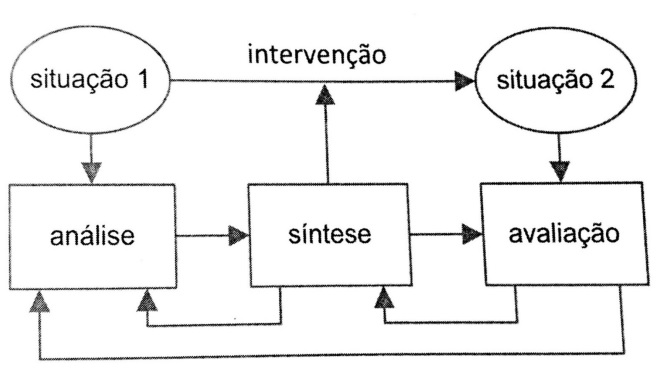
\includegraphics[width=\textwidth]{figuras/intervencao.jpg}
    \caption{Fluxograma do modelo de Análise de Situação e Síntese da Intervenção.}
    \label{fig_intervencao}
\end{figure}
\par
Este trabalho envolveu a co-criação com Alessio De Marchi. Alessio concebeu a ideia inicial do jogo e contribuiu para o design de algumas mecânicas e interações, bem como para a narrativa abordada pelo jogo. Além disso, ele forneceu os materiais artísticos necessários para a execução do jogo, conhecidos como \textit{Assets}. Durante a primeira reunião síncrona, foi definido o andamento do jogo, a quantidade de cenários presentes e quais seriam os inimigos presentes até aquele estágio. Posteriormente, outra reunião foi realizada para revisar o progresso e discutir possibilidades de adições ao jogo, como a inclusão de diálogos. Durante os meses seguintes, houve trocas de e-mails para atualizações do desenvolvimento e sugestões de novas adições ao produto final, a partir dos conceitos iniciais propostos por Alessio. Esses conceitos incluíam a possibilidade de melhorar as habilidades do personagem e a coleta de materiais, bem como a inclusão de laboratórios de desmonte e montagem nos cenários, conforme mencionado em documentos iniciais.
\par
%TODO
Cocriação é uma iniciativa de gestão, ou forma de estratégia econômica, que reúne diferentes partes (por exemplo, uma empresa e um grupo de clientes), a fim de produzir conjuntamente um resultado mutuamente valorizado \cite{PRAHALAD20045}. Podendo ser utilizado na frente do desenvolvimento de software, dentro de si, no desenvolvimento de jogos digitais, jogos digitais voltados para educação e saúde \cite{IHC_Estendido}, democraticamente inserindo pluralmente pessoas de amplas competências no desenvolvimento de um projeto complexo, "Participantes que jamais imaginaram-se usando um computador criaram seus jogos digitais. Participantes inicialmente inseguros com o uso de computadores começaram a ensinar outras pessoas a usarem para que pudessem jogar seus projetos." \cite{IHC_Estendido}.
\par
Um jogo chamado Par Tribus, desenvolvido por meio da cocriação, no Reino Unido, pela empresa Denki, por meio de\textit{feedbacks} de potenciais jogadores, minimizando riscos ouvindo-os, driblando um desperdício de material humano, de desenvolvimento técnico e evitar que apenas no final do desenvolvimento do jogo descobrir que ninguém o quer, isso ajudou a empresa a ter previsibilidade do seu produto \cite{lowthorpe2013stop}.
\par
Cocriação não é pedir aos clientes o que eles querem, mas sim, busca por \textit{feedback} criativo para soluções, para fazer uma entrega de valor agregado com o produto final e de participação conjunta, além de trazer uma visão sem viés técnico que desenvolvedores possuem. A multidisciplinaridade consegue se beneficiar da cocriação, pois consegue por meio da participação conjunta, trazer perspectivas plurais à concepção do que está sendo trabalhado, trazendo interações mais igualitárias e pelos participantes \cite{rock2018multidisciplinary}
\par
%TODO
Pela falta na literatura brasileira, de um trabalho que aborde o desenvolvimento de um jogo educacional que trata do problema causado pelos resíduos de materiais eletrônicos descartados de maneira incorreta, assim surge a proposta de um jogo digital, chamado What Weee Are, a ser inserido e apresentado à crianças e adolescentes em idade escolar, para auxiliar na aprendizagem, com a intenção de apresentar o risco da má gestão de resíduos de materiais eletrônicos, da falta de reciclagem. Jogos educacionais são uma ferramenta que pode ser utilizada para apresentação de conceitos de uma maneira interativa e lúdica às pessoas, além de ter sido identificado benefícios cognitivos e comportamentais do uso desta ferramenta \cite{gameUseOnSchool}, além de gerar curiosidade e interesse por parte daqueles que estão sendo apresentados, neste caso, crianças e adolescentes em idade escolar. \cite{savi2008jogos} 
\par
%TODO
What Weee Are é um projeto multimídia, um jogo eletrônico que aborda os desperdício de recursos de nossa sociedade, a ideia é que o jogo seja capaz de ser usado como uma ferramenta educacional a ser utilizada pelos professores, capaz de motivar o interesse dos alunos à reciclagem de materiais eletrônicos, um dos problemas atuais de nossa sociedade. Utilizar um jogo como ferramenta de educação já foi apresentado como viável e devemos aproveitar as oportunidades que o atual mundo tecnológico nos apresenta \cite{gameUseOnSchool}


\section{Justificativa}
\label{Justificativa}
Contudo, a partir de tudo isso, com os Objetivos de Desenvolvimento Sustentáveis da ONU para o Brasil \cite{odsbrasil}, e de como a educação é uma espaço onde existe a importância de levar conteúdos de impacto para o futuro e de como jogos sérios podem ser uma ótima ferramenta para ser utilizada no ensino e apresentação de conteúdos \cite{gameUseOnSchool}, de uma maneira mais dinâmica e ativa por parte dos alunos \cite{savi2008jogos}, e utilizando conceitos de Interação Humano-Computador para a concepção e desenvolvimento do projeto interativo \cite{IHC_Estendido}, por meio do fluxo de análise, síntese da intervenção e avaliação, da cocriação como ferramenta de desenvolvimento conjunto entre partes \cite{lowthorpe2013stop}. What Weee Are, propõe correlacionar estes três pontos junto com o problema dos resíduos de materiais eletrônicos no planeta.

\section{Objetivos}
\label{Objetivos}

\subsection{Objetivos Gerais}
% Objetivo geral é aplicar o co-design para o desenvolvimento de um sistema educativo
O objetivo do projeto acadêmico "What Weee Are" é desenvolver um jogo educativo utilizando técnicas de programação, boas práticas e estruturas de dados adequadas, com foco na conscientização sobre a importância da reciclagem de resíduos eletrônicos. O projeto também utiliza o co-design para permitir a participação dos usuários finais no processo de criação do sistema interativo e criar um produto que atenda às suas necessidades e expectativas.

O jogo será aplicado em escolas como uma ferramenta educativa para conscientizar os estudantes sobre a importância da reciclagem de resíduos eletrônicos e incentivar a sua participação nesse processo. Através da aplicação de conceitos de Interação Humano-Computador, o jogo será desenvolvido de forma clara e organizada para facilitar a manutenção e expansão futura do projeto.

\subsection{Objetivos Específicos}
No projeto What Weee Are, por meio da utilização do motor gráfico de desenvolvimento de jogos Unity como ferramenta de criação de jogos. O objetivo é permitir que os usuários interajam com o projeto de forma intuitiva e envolvente.

Para alcançar essa meta, é necessário empregar o motor gráfico de desenvolvimento de jogos Unity, que fornece recursos para criar experiências interativas e jogos. Essa plataforma é especialmente adequada para o projeto What Weee Are, pois disponibiliza de um ferramental abrangente para o desenvolvimento do projeto.

Além disso, para garantir a qualidade do projeto, é fundamental empregar técnicas de programação, aderir às melhores práticas e utilizar estruturas de dados apropriadas. A programação deve ser clara e organizada para simplificar a manutenção e expansão do projeto no futuro. As melhores práticas devem ser seguidas para garantir a segurança e eficiência do projeto. E as estruturas de dados devem ser escolhidas cuidadosamente para assegurar a escalabilidade e a eficiência no tratamento de grandes quantidades de dados.

O uso de técnicas como descrição do espaço de problemas, seleção de personas e cenários, bem como a análise hierárquica de tarefas são fundamentais para o desenvolvimento do jogo educativo What Weee Are. A descrição do espaço de problemas é uma técnica que permite identificar e delimitar os problemas ambientais relacionados ao descarte de resíduos eletrônicos. Isso ajuda a definir os limites do jogo e a direcionar a criação de desafios que abordem essas questões de forma realista e eficaz.

A seleção de personas é outra técnica importante, que permite definir as características e necessidades do público-alvo do jogo. Isso ajuda a criar personagens fictícios que representem diferentes perfis de jogadores, para que o jogo seja capaz de engajar e conscientizar pessoas de diferentes idades, gêneros e perfis socioeconômicos.

Os cenários, por sua vez, são as situações em que os personagens fictícios estão inseridos. Eles ajudam a contextualizar o jogo e a torná-lo mais atrativo e realista. Além disso, a análise hierárquica de tarefas é uma técnica que permite dividir as tarefas necessárias para completar o jogo em sub-tarefas menores, o que facilita o processo de criação e garante que o jogo seja consistente e bem estruturado.

Com o uso dessas técnicas, o What Weee Are poderá ser desenvolvido de forma apropriada, apresentando um enredo e personagens envolventes, desafios realistas e educativos e uma jogabilidade interessante e envolvente. O resultado final será um jogo educativo capaz de conscientizar jogadores sobre a importância do descarte correto de resíduos eletrônicos e os impactos positivos que essa prática pode trazer para o meio ambiente e para a sociedade como um todo.


\section{Organização de trabalho}
Este documento está organizado da seguinte forma:
1. Introdução (Capítulo 1): Este capítulo apresenta a motivação, justificativa, objetivos gerais e específicos da pesquisa, além de contextualizar o problema relacionado à educação em reciclagem de resíduos eletrônicos.

2. Trabalhos Relacionados (Capítulo \ref{trabalhos relacionados}): Neste capítulo, são discutidos trabalhos e pesquisas anteriores sobre o tema, proporcionando um panorama sobre o estado da arte no campo de estudo e apontando possíveis lacunas na literatura.

3. Ferramentas (Capítulo \ref{ferramentas}): O Capítulo 3 descreve as ferramentas e tecnologias utilizadas para o desenvolvimento do jogo educativo "What Weee Are", incluindo a plataforma Unity, as linguagens de programação empregadas e os formatos de jogo.

4. Desenvolvimento (Capítulo \ref{desenvolvimento} e \ref{desenvolvimento_tecnico}): Estes capítulos explora os métodos e técnicas aplicadas no processo de desenvolvimento do jogo, abordando a descrição do espaço de problemas, seleção de personas e cenários, e a análise hierárquica de tarefas, são apresentados conceitos de Interação Humano-Computador, que ajudam a contextualizar a apresentação do projeto e embasar as escolhas de design e implementação do jogo.  O Capítulo \ref{desenvolvimento_tecnico} traz uma discussão sobre os conceitos técnicos abordados no trabalho, contribuindo para a compreensão dos aspectos fundamentais envolvidos no desenvolvimento do projeto "What Weee Are".
